\documentclass[twocolumn]{article}
\usepackage[top=1in, bottom=1in, left=1in, right=1in]{geometry}
\usepackage{graphicx}
\usepackage{cite}
\begin{document}

\title{Organ Sound Synthesis by Harmonic Interpolation}
\author{Matthew W. Jibson}

\maketitle{}

\begin{abstract}

Synthetic sound generation techniques for pipe organs are currently based on samples and wave tables, and physical synthesis. The samples require expensive and time-consuming editing and recording. In this paper I present a method of synthesizing pipe organ sounds using additive synthesis by interpolating certain harmonics of recordings. The $N$ largest frequency components of the power spectral density of each recording are found and analyzed to find their percentage power contribution to the overall recording and harmonic above the fundamental. Simple polynomial fit algorithms are applied to each of the $N$ components and a function generated to describe them at any frequency. Unique sinusoids can be generated in real time at arbitrary frequencies and amplitudes without the need for samples or wave tables.

\end{abstract}

\section{Introduction}

Current sound-generation techniques for organs generally involve some combination of (1) playback of pre-recorded samples or wave tables, (2) sampling playback manipulation or interpolation to adjust pitch, (3) physical models describing pipe output. The first method, which requires organ tuning, recording, and editing of samples sets is expensive, time consuming, data intensive, and limits playback to only recorded pitches. The second method, when combined with the first, allows any pitch to be produced, but only at exact harmonic structure as the original sample. The third method, though inexpensive and appropriate for real time work, does not take into account slight variations in pipe construction across the range, and so again results in a static harmonic structure. Hence, no current method is inexpensive, easily available, and accurate to organ acoustics.

This paper presents a method to address these shortcomings by proposing a relatively simple, inexpensive approach to model a harmonic structure across an entire range. This method requires only a limited number of recordings, which need not be of high quality or in tune. A set of continuous functions is produced, which will be able to generate unique outputs at any frequency.

\section{Background}

A piano and a violin, when playing the same note (i.e., sounding the same pitch), are distinguishable because of the harmonic structure of the created sound. When a specific note is played, resonance occurs, producing a sound at a specific base or fundamental frequency. Additional frequencies that are positive integer multiples of that base frequency also are produced. These frequencies are called the harmonic series. For example, if a note is played with a base frequency of 200Hz, harmonics at 400Hz, 600Hz, etc.\ are also produced. Some instruments only generate the odd harmonics: from the base of 200Hz, 400Hz is skipped and 600Hz remains, etc. The trend of these harmonics is to decrease in power as distance from the base frequency increases. Other frequencies that are not positive integer multiples are also produced with, in general, much lower power, but with a similar decreasing trend. Hence, these differences in harmonic structure produced aural (heard) differences between instruments.

Pipe organs are unique wind instruments in that each sound is generated by its own pipe. This, by nature, creates variations in the harmonics of each pipe (and thus over the entire range) because of slight fabrication differences or purposeful voicing differences by the builder. This is in contrast with other wind instruments where the effective length of a single pipe is changed with valves (e.g., trumpet), holes that are covered (e.g., clarinet), or a slide (e.g., trombone). Thus, other wind instruments, which are based on a single piece of metal or wood, have a similar harmonic structure over their entire range.

\section{Method}

\subsection{Recording Analysis}

Recordings of the chosen notes are made and edited to include only the primary pipe speech, excluding the initial attack and final release of the note where other effects occur (Figure \ref{time}). The power spectral density of each recording is estimated (e.g., using Welch's method \cite{welch-psd}, Figure \ref{peaks}). A PSD function determines the power distribution of a signal in the frequency domain. This allows determination of the power of the signal at discrete frequencies. The $N$ (an arbitrary number chosen by the user) largest peaks in each distribution are found by searching for three consecutive points where the middle point has greater value than both surrounding points (Figure \ref{peaks}). The percentage power contribution of each peak is found by dividing the power of the peak by the total power of the distribution. Finally, the expected base frequency is recorded as the closest frequency to it that is also one of the $N$ peaks. The exact base frequency cannot be used because the PSD function produces a list of discrete frequencies. Furthermore, the number of peaks is chosen so that there is a close match (within 2Hz, generally). This is generally not an issue because the base frequency is almost always one of the first two peaks.

\begin{figure}
\centering
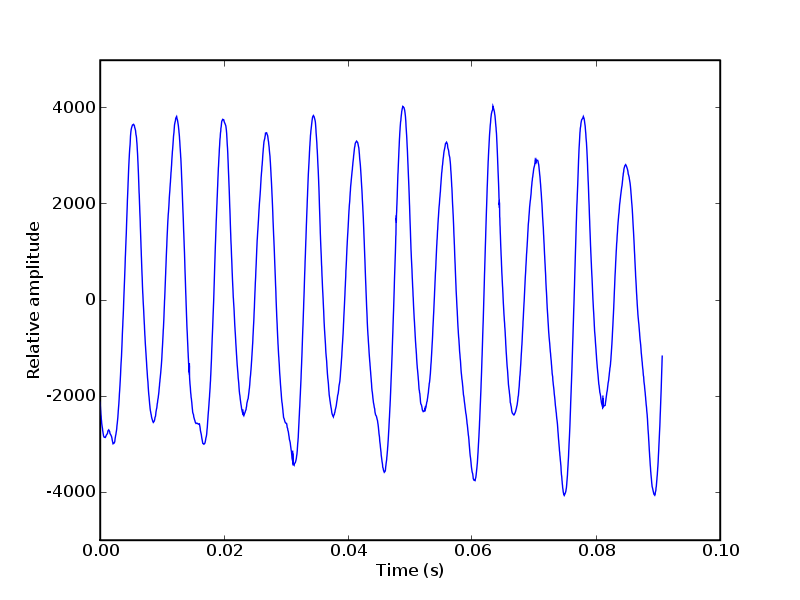
\includegraphics[width=\linewidth]{figures/recording-time.png}
\caption{Excerpt of a recorded wave.}
\label{time}
\end{figure}

\begin{figure}
\centering
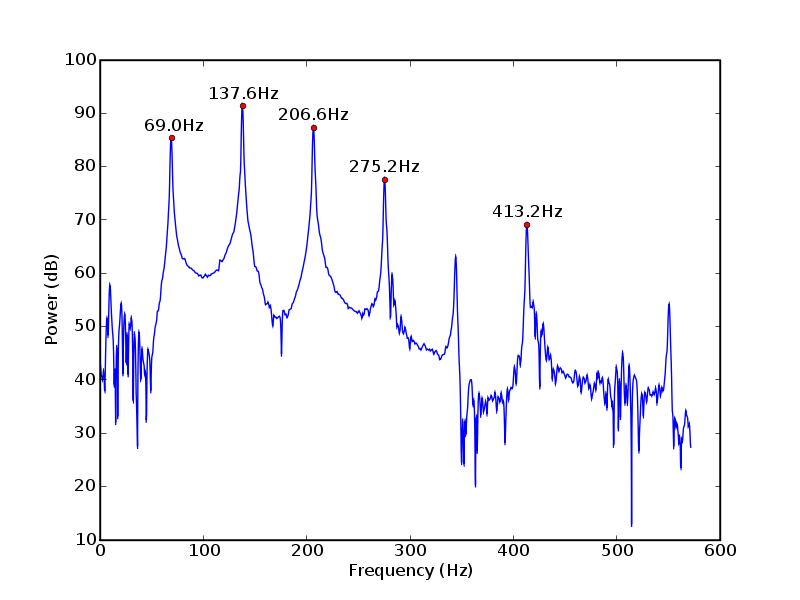
\includegraphics[width=\linewidth]{figures/recording-peaks.png}
\caption{Excerpt of the PSD of a recorded wave. The first five peaks are marked with red circles.}
\label{peaks}
\end{figure}

At this point processing on individual recordings is complete, and they can now be processed as a set. The first peak power contribution of each recording is taken, along with that recording's base frequency. A least-squares polynomial fit algorithm is applied where the base frequency ($F$) is the independent variable and the peak power contribution corresponding to that base frequency ($P$) is the dependent variable. Third-degree polynomials tend to produce good results. This procedure is repeated for all of the other $N$ peaks so that the polynomial fit algorithm is applied to all of the second, third, etc.\ peak power contributions up to $N$. These algorithms generate coefficients $a$, $b$, and $c$ for the simple polynomial \begin{equation} \label{eq:power} P = aF^2 + bF + c,\end{equation} where $F$ is the desired frequency and $P$ is the resultant power contribution for each of the first $N$ power contributions. This produces continuous functions from which to generate individual (and likely unique) harmonic structures at any frequency.

\subsection{Sound Synthesis}

To synthesize a desired sound at base frequency $F$Hz, find the frequencies of the $N$ peaks of the recording with the closest base frequency to $F$. Alternatively, other search methods can be used. For example, find the recording with the closest base frequency to $F$ that is not greater than $F$, if there is such a frequency. Generate sinusoids at these frequencies at desired lengths and sampling frequencies. Apply $F$ to Eq. (\ref{eq:power}) with output as $P$, and scale (e.g., multiply) each value from the generated sinusoids by $P$. Then simply add the first, second, third, etc.\ value of each wave together to produce the output wave.

\section{Results}

One test of this method involved recordings of five C$\sharp$s of the 8-foot principal rank (C$\sharp$1 to C$\sharp$5). The lowest recording, which has a base frequency of 137.16Hz, was used as a reference for comparison (Figures \ref{time}--\ref{peaks}). Using the above method a wave was synthesized (Figure \ref{synth-time}). The resulting PSD from the synthesized wave (Figure \ref{synth-peaks}) shows peaks with similar frequencies and amplitudes to the reference. Clearly all of the other features of the wave (non-smoothness between peaks of Figure \ref{peaks}) are lost and not generated in this synthesized wave.

\begin{figure}
\centering
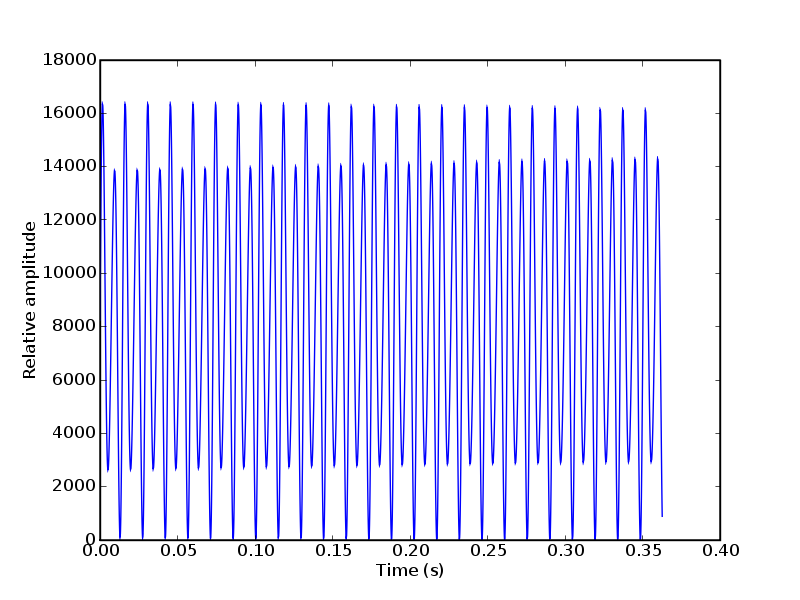
\includegraphics[width=\linewidth]{figures/synth-time.png}
\caption{Excerpt of a synthesized wave.}
\label{synth-time}
\end{figure}

\begin{figure}
\centering
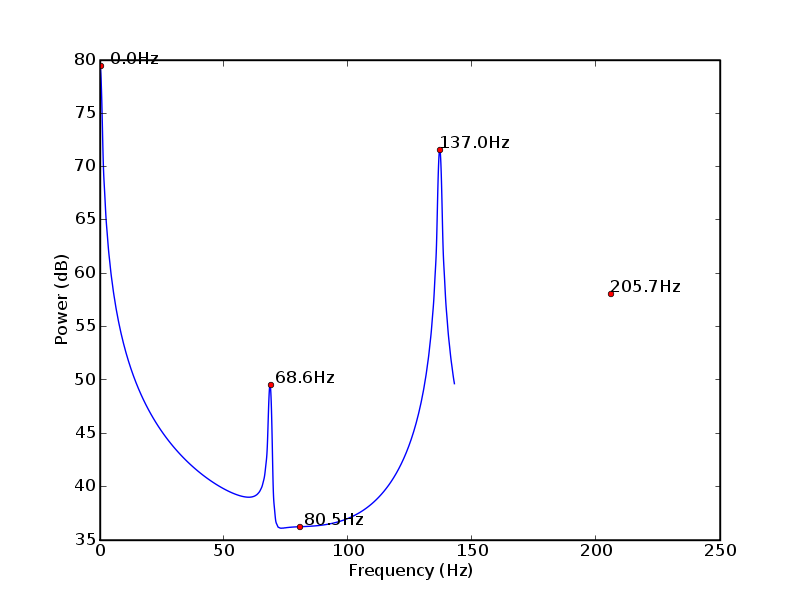
\includegraphics[width=\linewidth]{figures/synth-peaks.png}
\caption{Excerpt of the PSD of a synthesized wave. The first five peaks are marked with red circles.}
\label{synth-peaks}
\end{figure}

Listening test results are acceptable. The produced sound is clearly of correct pitch and timbre. It is also, however, clearly computer generated. This is expected because, as noted above, all features outside of the generated peaks are lost. Furthermore, when going beyond the range of the lowest and highest recorded sounds, the generated sounds can get wildly inaccurate, with the percentage contribution multipliers quickly blowing up, yielding meaningless results. Thus, generated sounds should be confined to the interval between the lowest and highest recorded notes, or within a small margin thereof.

As a result of using the closest recorded note to the desired frequency as the basis for the harmonic structure, there are very noticeable changes when listening to a full range sweep of produced noises (i.e., a generated tone corresponding to each note on an organ). This occurs when the closest recorded note switches to another recorded note. The change in harmonic structure is noticeable since it is so abrupt and unnatural.

Regarding a computer back end, this method meets the requirements of real time speed. Generating sinusoids at a certain sampling frequency (e.g., 48kHz) for $N$ peaks (e.g., 50) is about 2.4 million samples per second. Each sample requires a sinusoid operation, two multiplication operations, and some trivial operations that have no significant performance effect. Modern computers run in the range of billions of operations per second, or about two to four orders of magnitude faster than required to process real-time requests of a naive implementation. There is thus computational availability for multiple notes. With optimized, cached, or preprocessed data, this availability can increase further. For example, ChucK can easily mix 100 sinusoids at 44.1kHz on the author's computer, which has a clock rate of 2.0 GHz.

Processing speed of this algorithm is on the order of one second per recording. The author's implementation in Python is slowest at searching for peaks after a PSD has been performed. The PSD function, which involves many Fast Fourier Transforms (FFT), is not computationally expensive. In order to increase frequency precision, the number of FFT points is high ($2^{17}$), which is larger than the number of samples in most recordings under 2 seconds, and thus only one FFT is computed per recording. However, computation time is not a critical issue because it need only be done once and can be done when time constraints are lenient.

\section{Discussion and Further Work}

As touched on above, there are some boundaries between notes on a full range where the harmonic structure noticeably changes from one recorded note's structure to another's. It is not possible simply to apply a polynomial fitting algorithm to the harmonics as was done in the power contribution case. For example, consider a set consisting of two recordings of C1 and C2 (which are an octave apart). Both recordings have as their most powerful frequency (first peak) their base frequency. The lower recording has as its second most powerful frequency (second peak) twice the base frequency (one octave or $12/12^\mathrm{ths}$ above the base), as would be expected from a simple harmonic series. The higher recording, however, has as its second peak triple the base frequency (two octaves or $24/12^\mathrm{ths}$ above the base). If a simple linear interpolation is applied to determine the second peaks, the results between C1 and C2 will evenly distribute between $12/12^\mathrm{ths}$ and $24/12^\mathrm{ths}$ above the base, which frequencies are not in the harmonic series, and thus will not sound correct. For example, taking one note above the lowest recording, C$\sharp$1, this incorrect interpolation dictates the second peak should be $13/12^\mathrm{ths}$ above the base. D1 similarly has a second peak $14/12^\mathrm{ths}$ above the base, continuing up to B1 at $23/12^\mathrm{ths}$, and ending at C2 at $24/12^\mathrm{ths}$ above the base, or triple the base frequency.

In general, the harmonics above the base are taken from a set of often-used harmonics, that tend to be integer multiples above or integer divisors below (e.g., $1/2$) the base frequency. Thus, a solution is perhaps a somewhat discretized list assigning a certain probability to each harmonic. Other algorithms involving optimization and genetic algorithms may suggest other models. These models, when applied to data from a recording set over a full range of notes, could yield methods to generate individual harmonic structure for all frequencies.

Of interest to sound engineers and others interested in vocoders is the possibility of applying this method on a recording set not consisting of all one instrument. For example, a recording set of a bass drum, oboe, and voice could produce unique results with varying components of each at all ranges. This application, however, is not worth while until the harmonic structure is a function of frequency, as discussed in the proceeding paragraph.

The method described herein does not model many parts pipe speech: (1) the beginning of pipe speech, called chiff, is an important part of all pipe organs that is specifically modified (not removed) by the builder during installation; (2) the end of pipe speech, which is of less importance; (3) sibilance, the sound of air moving over a pipe mouth during nominal speech. Without these it is clear that the produced sound does not come from a genuine pipe. The above method works well on sounds that have a few significant frequencies making up much of the sound. These three parts of pipe speech have no such property, and so are perhaps modeled better in the time domain, instead of the frequency domain.

\section{Conclusion}

Current sound synthesis techniques are computationally and monetarily expensive, and harmonically identical. The method presented above for organ sound synthesis produces functions that can describe unique waveforms at arbitrary frequencies within the range of the recordings. Since many parts of pipe speech are not modeled and other harmonic problems remain, this method is not fit for use in production systems. However, the results show a working proof-of-concept implementation, and suggest further work is warranted.

The author has implementations available online in Python, which outputs a ChucK file, and MATLAB, which outputs wav files (http://mattjibson.com/schalmei/).

\bibliography{paper}{}
\bibliographystyle{ieeetr}

\end{document}
